% Created 2018-11-14 Wed 15:43
% Intended LaTeX compiler: pdflatex
\documentclass[11pt]{article}
\usepackage[utf8]{inputenc}
\usepackage[T1]{fontenc}
\usepackage{graphicx}
\usepackage{grffile}
\usepackage{longtable}
\usepackage{wrapfig}
\usepackage{rotating}
\usepackage[normalem]{ulem}
\usepackage{amsmath}
\usepackage{textcomp}
\usepackage{amssymb}
\usepackage{capt-of}
\usepackage{hyperref}
\setcounter{secnumdepth}{3}
\author{Kenneth Yan}
\date{\today}
\title{ExtractTF\\\medskip
\large Extract Titles and Footnotes from DPS - Part 1}
\hypersetup{
 pdfauthor={Kenneth Yan},
 pdftitle={ExtractTF},
 pdfkeywords={},
 pdfsubject={},
 pdfcreator={Emacs 26.1 (Org mode 9.1.9)}, 
 pdflang={English}}
\begin{document}

\maketitle
\setcounter{tocdepth}{2}
\tableofcontents

\section{Introduction}
\label{sec:org3607aed}
ExtractTF is a tool to extract the titles and footnotes from the Word document of Data Presentation Specifications - Part 1(.docx), then export them to .XLSX or .XML file which can be transfered to SAS dataset easily.

\begin{figure}[htbp]
\centering
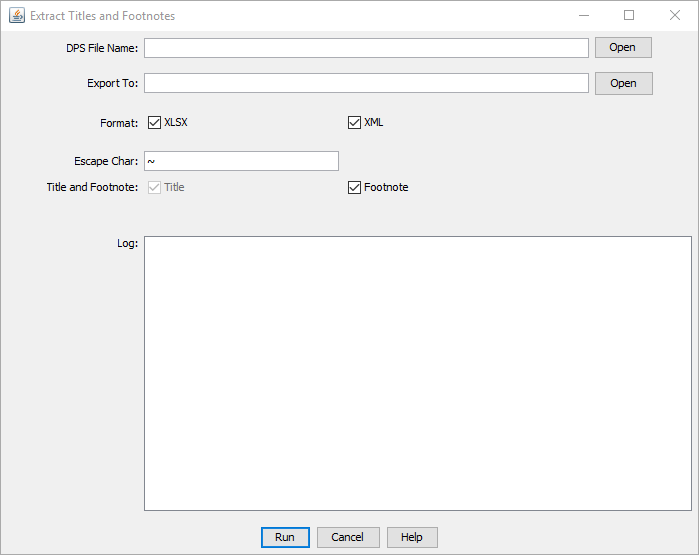
\includegraphics[width=.9\linewidth]{./images/001.png}
\caption{The window of ExtractTF}
\end{figure}

\subsection{Key Elements to extract from DPS}
\label{sec:orga8eff2a}

\begin{itemize}
\item Study ID
\end{itemize}
The study ID is extracted from the first page of DPS - Part 1. See the picture below. 
\begin{figure}[htbp]
\centering
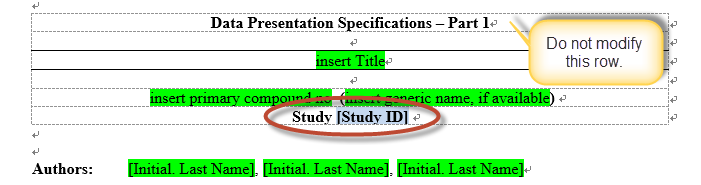
\includegraphics[width=.9\linewidth]{./images/002.png}
\caption{Study ID}
\end{figure}

\begin{itemize}
\item Title
\item Analysis Set
\end{itemize}
\begin{figure}[htbp]
\centering
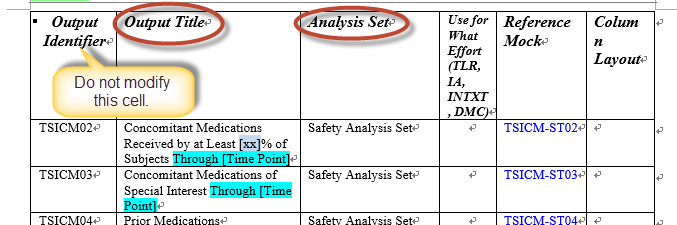
\includegraphics[width=.9\linewidth]{./images/003.png}
\caption{Title and Analysis Set}
\end{figure}


\begin{itemize}
\item Footnote
\end{itemize}
The footnotes \textbf{is} extracted from the \textbf{Display Specifications} table, and \textbf{is not} extracted from the shell table. See the picture below.
\begin{figure}[htbp]
\centering
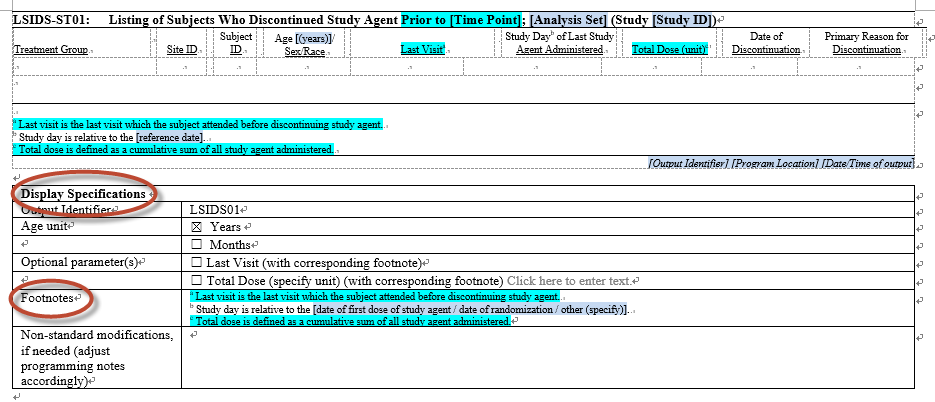
\includegraphics[width=.9\linewidth]{./images/004.png}
\caption{Footnotes}
\end{figure}

\section{Install}
\label{sec:org1be2de9}
Copy the folder \texttt{S:\textbackslash{}2\_Tools\textbackslash{}ExtractTF} to your desktop, such as \texttt{C:\textbackslash{}ExtractTF}.

\section{Step by step guide}
\label{sec:org66604bc}

\subsection{Run ExtractTF}
\label{sec:orgff9b9c5}
Double click the file \textbf{ExtractTF.jar} to run. 

\subsection{Define "DPS File Name"}
\label{sec:orgdcf1ca0}
Click the "Open" button to select the DPS file from which you want to extract the titles and footnotes.

\subsection{Define "Export To"}
\label{sec:org4f6ab70}
Click the "Open" button to select the folder that Titles.xlsx/Titles.xml will save to. 

\subsection{Define "Format"}
\label{sec:org22c047e}
By default, both XLSX and XML are selected. You can make the change per your need.

\subsection{Define "Escape Char"}
\label{sec:org9784bb0}
By default, the escase char is '\textasciitilde{}'. You can change it to other char if needed.
This escape char is often used by superscript char, such as \emph{\textbf{\textasciitilde{}\{super a\}} p-value is from a log-rank test stratified by ECGO PS score (0 or 1) and age group (<65 or >=65).}

\subsection{Select "Title and Footnote"}
\label{sec:orgccf5a10}
Be default, both titles and footnotes are checked. If you do not need the footnotes information, you can uncheck its checkbox.

\subsection{Click "Run" button.}
\label{sec:orgd845906}
You can see the log info while it is running. 

\section{Transfer to SAS dataset}
\label{sec:org0719498}
\subsection{Import Titles.xlsx file}
\label{sec:orgd325e5a}
Use the global reporting macro \%RMDPSTITLE to import Titles.xlsx file.

\subsection{Import Titles.xml file}
\label{sec:org46718c2}
Use the SAS code below to import Titles.xml. You can find the code in the file \emph{ExtractTF\ImportXML.sas}.

\begin{verbatim}
libname temp xml "c:\D\temp\Titles.xml"; /* Change the path of Titles.xml */

data titles;
    set temp.titles;
run;

\end{verbatim}

\section{Support Information}
\label{sec:org3c2619b}
\begin{info}
Please write Email to: \\

\href{mailto:DL-RNDUS-GCDO-IDAR-SP-AI@ITS.JNJ.com}{DL-GCDO-IDAR-SP-AI}
\end{info}
\end{document}
